Adding derived density reduces cycle complexity in the joint space, suggesting that density acts as a regularizing coordinate rather than introducing additional branching. Results are lens-sensitive; pca2 should remain the primary interpretation layer, while density/domain are sensitivity probes.

\begin{figure}[H]
\centering
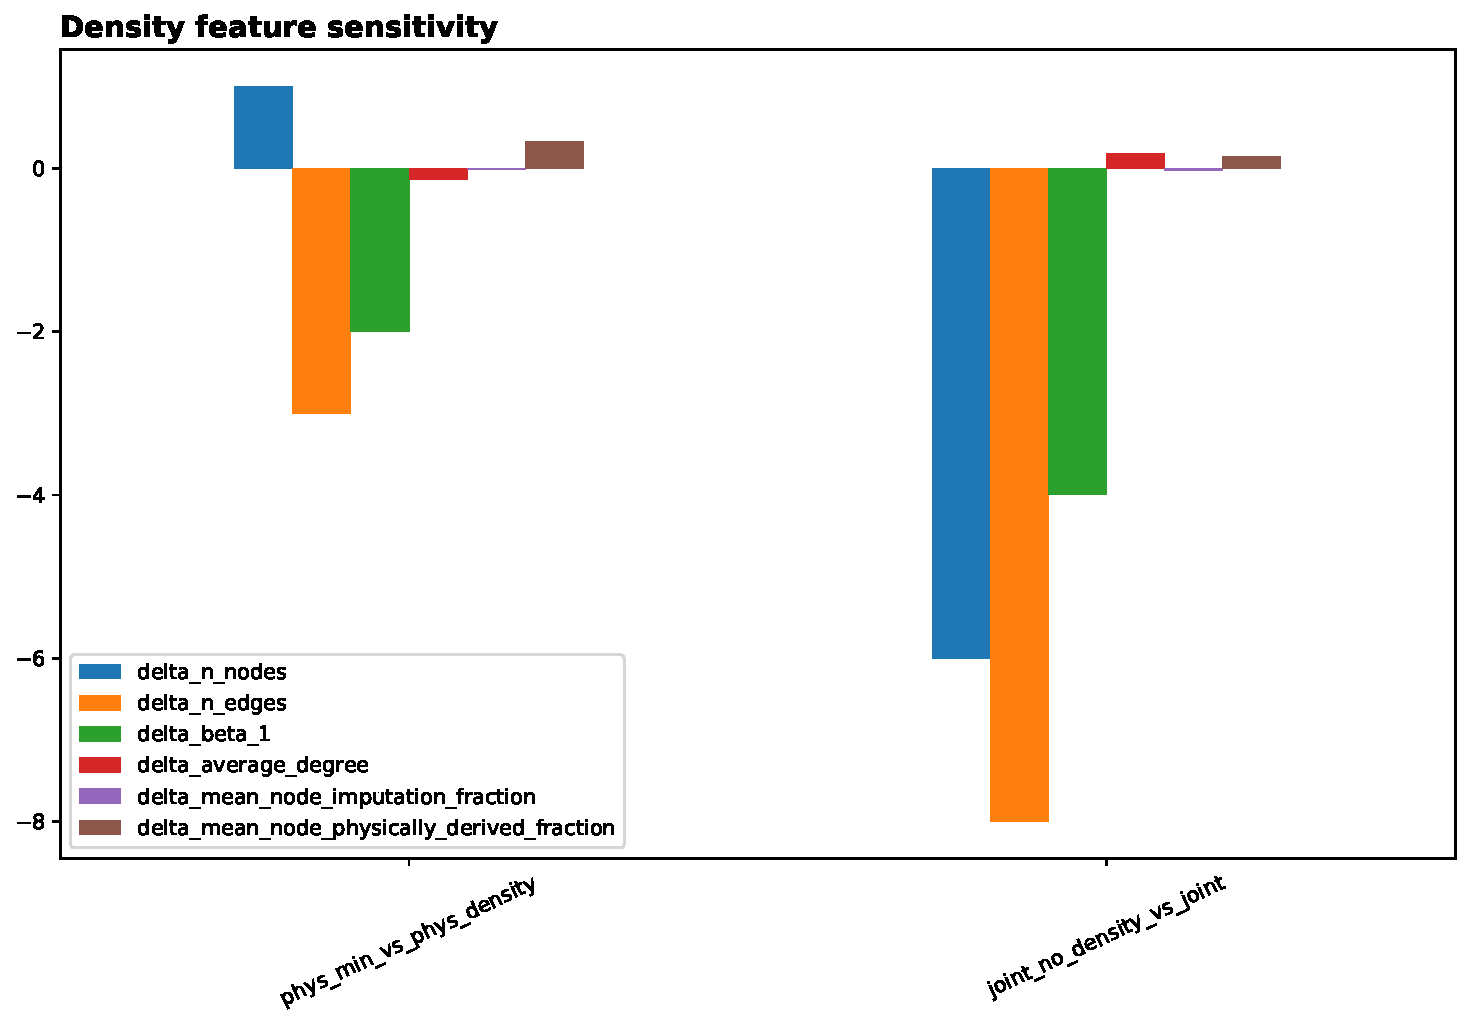
\includegraphics[width=0.9\linewidth]{figures/06_mapper_density_feature_sensitivity.pdf}
\caption{Sensibilidad al agregar pl\_dens.}
\end{figure}

La Figura 9 es una de las mas limpias del reporte porque la direccion del efecto es consistente en ambas comparaciones. Al agregar \texttt{pl\_dens}, los cambios dominantes son negativos en aristas y en $\beta_1$. En el espacio conjunto la reduccion es mas marcada, lo que sugiere que la densidad no abre nuevas ramas sino que colapsa parte de la geometria al introducir una coordenada derivada de masa y radio. Dicho de otra forma: la densidad organiza mejor, pero tambien puede volver menos independiente la lectura estadistica.

\begin{figure}[H]
\centering
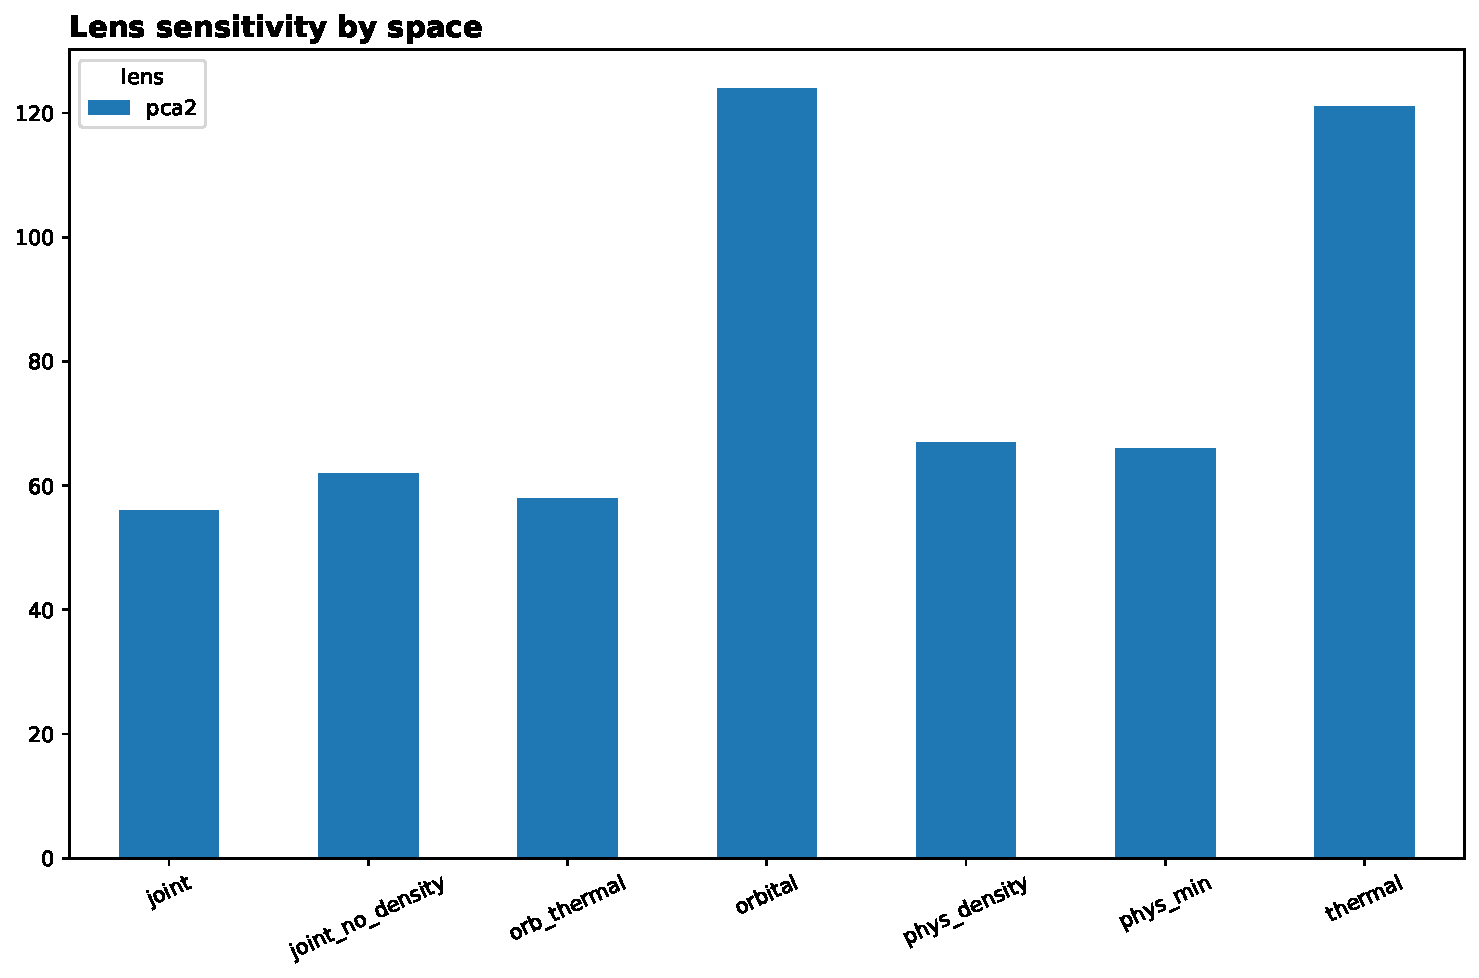
\includegraphics[width=0.9\linewidth]{figures/07_mapper_lens_sensitivity.pdf}
\caption{Sensibilidad al lens.}
\end{figure}

La Figura 10 confirma que la complejidad depende del espacio analizado y que el lens no debe verse como un detalle tecnico menor. Aun cuando aqui se resume solo la corrida con \texttt{pca2}, la dispersion entre espacios deja claro que el comportamiento de Mapper cambia mucho segun la proyeccion elegida. Por eso conviene mantener a \texttt{pca2} como lens principal de lectura y usar otras lentes como pruebas de sensibilidad, no como reemplazo directo de la interpretacion base.

\begin{figure}[H]
\centering

\includegraphics[width=0.9\linewidth]{figures/11_imputation_method_comparison.pdf}
\caption{Comparacion entre metodos de imputacion cuando esta disponible.}
\end{figure}

La Figura 11 ayuda a poner en contexto la robustez del pipeline frente al metodo de imputacion. El mensaje visual no es que todas las barras coincidan exactamente, sino que las configuraciones prioritarias no colapsan por completo cuando cambia la estrategia de completacion. Si una configuracion conserva orden de magnitud en nodos y ciclos entre metodos, entonces su lectura exploratoria gana credibilidad. Si cambia demasiado, debe tratarse como una dependencia metodologica y no como un rasgo fisico del catalogo.
